\documentclass[conference]{IEEEtran}
\usepackage{amsmath,amssymb,amsfonts}
\usepackage{graphicx}
\usepackage{booktabs}
\usepackage{array}
\usepackage{xcolor}
\usepackage{cite}
\usepackage{textcomp}
\usepackage{algorithm}
\usepackage{algpseudocode}
\usepackage{tikz}
\usetikzlibrary{positioning,shapes.geometric,arrows.meta,fit,backgrounds,calc}
\usepackage[hidelinks]{hyperref}

% ---------- shared definitions ----------
\newcommand{\authblock}[2]{\begin{minipage}[t]{0.31\textwidth}\centering
{\large #1}\\[0.5ex]
\footnotesize\textit{School of Computing Science and}\\
\footnotesize\textit{Engineering, VIT Bhopal University}\\
\footnotesize Sehore, Madhya Pradesh, India\\
\footnotesize #2
\end{minipage}}
% Numbers written by scripts/06_paper_benchmark.R (nTrain, nTest, bestAUC, ...)
\newcommand{\nTrain}{14{,}408}
\newcommand{\nTest}{4{,}803}
\newcommand{\posShare}{81.2}
\newcommand{\baselineAcc}{0.812}
\newcommand{\bestModel}{XGBoost}
\newcommand{\bestAUC}{0.666}
\newcommand{\bestAUCci}{0.647--0.685}
\newcommand{\bestAcc}{0.575}
\newcommand{\bestFone}{0.676}
\newcommand{\bestRecall}{0.548}
\newcommand{\bestSpec}{0.691}
\newcommand{\bestMCC}{0.186}
\newcommand{\bestDeltaAUC}{+0.010}
\newcommand{\bestDeltaP}{0.042}
\newcommand{\lrAUC}{0.656}
\newcommand{\lrAcc}{0.585}
\newcommand{\rfAUC}{0.634}
\newcommand{\rfAcc}{0.608}
\newcommand{\nModels}{6}

\renewcommand{\arraystretch}{1.1}

\begin{document}

\title{Do Developers Trust AI? Adoption, Trust and Pay in the 2025 Stack Overflow Survey}

\author{%
\begin{minipage}{\textwidth}\centering
\authblock{Manikandan J}{jdkmani@gmail.com}\hfill
\authblock{Narendren S V}{narendren2006@gmail.com}\hfill
\authblock{Murugavel J}{jmurugavel778@gmail.com}\\[1.2ex]
\authblock{Akash}{ak05ash20@gmail.com}\hfill
\authblock{Bharath}{bharathbps01@gmail.com}\hfill
\authblock{Disoor S}{sdisoor@gmail.com}
\end{minipage}}

\maketitle

%==================================================================
\begin{abstract}
Generative AI tools have become routine in software development, but it is unclear whether their widespread use has been matched by trust or by higher pay. This paper analyses the Stack Overflow Annual Developer Survey 2025 (49{,}191 responses, 172 variables), which is reduced to 44{,}682 professional developers from 175 countries after cleaning. The analysis combines hypothesis tests with effect sizes and Holm correction, salary regression with robust and inverse-probability-weighted estimates, an ordinal model of trust, a benchmark of six classifiers for AI adoption, and k-means clustering with resampling stability. Among respondents who answered each question, 79.4\% of professionals use AI tools and 48.1\% use them daily, yet only 32.4\% trust their accuracy. Adoption falls from 88.5\% among developers with 0--2 years of experience to 72.7\% among those with 20 or more. AI users earn less on average (median \$76{,}097 against \$81{,}685; Cohen's $d=-0.16$), but the AI-use coefficient is not significantly different from zero once experience, region and other covariates are controlled. Adoption is only weakly predictable: across six benchmarked models the best test AUC is \bestAUC{} (\bestModel), and its advantage over logistic regression is not significant after Holm correction. Clustering yields two attitude groups that are stable under resampling (mean adjusted Rand index 0.998). Adoption, trust and pay are largely separate matters, and with samples this large, effect sizes are more informative than $p$-values.
\end{abstract}

\begin{IEEEkeywords}
AI adoption, developer survey, trust in AI, hypothesis testing, ordinal regression, ROC analysis, k-means clustering, Stack Overflow.
\end{IEEEkeywords}

%==================================================================
\section{Introduction}
AI coding assistants have become common in professional software development within a few years. Controlled experiments suggest that they can speed up programming tasks \cite{peng2023}, which raises two practical questions: whether developers trust the output, and whether using the tools is rewarded financially. Large annual surveys such as the Stack Overflow Developer Survey \cite{so2025} give a broad view of how developers use and judge these tools. Answering them takes more than descriptive percentages: the data are observational, self-selected and partly missing, and the samples are so large that almost any difference is statistically significant.

This study addresses six research questions:
\begin{itemize}
\item \textbf{RQ1} Does AI tool adoption depend on developer role and experience?
\item \textbf{RQ2} Do AI users earn more than non-users?
\item \textbf{RQ3} Does trust in AI accuracy change with experience?
\item \textbf{RQ4} Can AI adoption be predicted from professional attributes?
\item \textbf{RQ5} Are there distinct developer ``personas'' in AI attitudes?
\item \textbf{RQ6} What predicts \emph{how much} a developer trusts AI on the five-point scale?
\end{itemize}

The main contributions of this paper are:
\begin{itemize}
\item A scripted, seeded R pipeline that runs from the raw survey file to the final report. The benchmark tables and figures in this paper are written directly by the code.
\item Effect-size-based inference: Cram\'er's $V$, Cohen's $d$, $\eta^2$ and the rank-biserial correlation are reported alongside Holm-adjusted $p$-values and explicit assumption checks.
\item Robustness checks on the headline results (HC3 standard errors, inverse-probability weighting, proportional-odds checks and cluster resampling).
\item A benchmark protocol (Algorithm~\ref{alg:bench}) that compares six models for adoption prediction using confusion matrices, ROC/AUC with confidence intervals and significance tests.
\item A two-group segmentation of AI attitudes that is stable under resampling and is checked against variables not used in the clustering.
\end{itemize}

%==================================================================
\section{Existing Work}

\subsection{Developer Surveys and AI Productivity}
Controlled experiments with GitHub Copilot report that developers complete a bounded programming task considerably faster with the tool \cite{peng2023}. Such experiments measure speed on a defined task, whereas survey data add the developers' own view: the most common frustration in the survey analysed here is output that is almost right but not quite \cite{so2025}. This paper examines adoption, trust and pay together in one global professional sample. Because survey respondents are self-selected, causal claims cannot be supported, and the paper reports associations only.

\subsection{Statistical Inference with Large Samples}
With tens of thousands of observations, $p$-values are almost always small, so interpretation rests on effect sizes. Cohen's $d$ \cite{cohen1988} is the usual choice for mean differences and Cram\'er's $V$ for contingency tables. Families of tests can be controlled with Holm's step-down procedure \cite{holm1979}. When the residual variance is not constant, the Breusch--Pagan test \cite{breusch1979} and HC3 covariance estimators \cite{white1980,mackinnon1985} provide valid standard errors. Ordered responses are commonly modelled with the proportional-odds model \cite{mccullagh1980,agresti2010}, and non-response in an outcome can be addressed with inverse-probability weighting \cite{seaman2013}.

\subsection{Machine Learning for Tabular Data}
Random forests \cite{breiman2001} remain a strong baseline for tabular problems. Gradient-boosted trees such as XGBoost \cite{chen2016}, LightGBM \cite{ke2017} and CatBoost \cite{prokhorenkova2018} are widely used in applied work, and comparative studies find that tree-based models still match or beat deep networks on medium-sized tabular data \cite{grinsztajn2022,shwartz2022}. Deep tabular architectures such as FT-Transformer \cite{gorishniy2021} and TabTransformer \cite{huang2020}, and pre-trained models such as TabPFN \cite{hollmann2025}, are active research areas. Models can be compared on a held-out set using ROC analysis \cite{fawcett2006}, DeLong's test for correlated AUCs \cite{delong1988} and McNemar's test for paired error rates \cite{mcnemar1947}.

\subsection{Unsupervised Segmentation and its Validity}
The k-means algorithm \cite{macqueen1967} is widely used to segment survey respondents, but the result is only useful if the structure it finds is real. Silhouette width \cite{rousseeuw1987} measures how well separated the clusters are, whereas the adjusted Rand index \cite{hubert1985} measures how reproducible they are under resampling.

\subsection{Design Requirements and Contributions}
Four requirements follow from the methods reviewed above. First, results must be reported with effect sizes and robustness checks, not with $p$-values alone. Second, adoption, trust and pay must be analysed together in a single sample. Third, models for adoption prediction must be compared on a common split with threshold-aware metrics and significance tests. Fourth, any segmentation must be accompanied by a stability analysis. The pipeline, benchmark and robustness analysis described in the next section are designed to meet these requirements.

%==================================================================
\section{Proposed Methodology}

\subsection{Dataset Description}
The data come from the Stack Overflow Annual Developer Survey 2025 \cite{so2025}, which is released under CC BY-SA 4.0. The raw file contains 49{,}191 responses and 172 columns from 175 countries. Restricting the sample to respondents who are developers by profession or who write code as part of their work leaves 44{,}682 respondents from 175 countries, and feature engineering yields 38 analysis columns. Table~\ref{tab:dataset} summarises the dataset and Table~\ref{tab:features} lists the predictors used for adoption prediction.

\begin{table}[t]
\caption{Dataset summary and preprocessing decisions}
\label{tab:dataset}
\centering
\small
\begin{tabular}{@{}p{2.2cm}p{5.5cm}@{}}
\toprule
\textbf{Property} & \textbf{Value / treatment} \\
\midrule
Raw size & 49{,}191 rows $\times$ 172 columns \\
Analysis sample & 44{,}682 professional developers (developers by profession or coding as part of their work) \\
Countries & 175 in the analysis sample, collapsed to 7 regions \\
Analysis columns & 38 after feature engineering (AI usage, trust and sentiment scores, role, experience, age, education, organisation size, region, remote work, job satisfaction, salary, language and AI-model counts) \\
Experience & \texttt{YearsCode} text converted to numeric \\
Age & age buckets converted to midpoints \\
Education, org.\ size & 8 $\to$ 4 and 9 $\to$ 3 categories (``No degree'' to ``Doctorate/Professional''; small, medium, large) \\
Salary & \texttt{ConvertedCompYearly}; values $<\$1{,}000$ or above the 99th percentile \emph{flagged, not deleted}; modelled as $\log$(salary) \\
Salary availability & 52.1\% report pay; rate varies by region \\
Multi-select fields & counted for breadth (languages, AI models) and split into one row per answer for frequency charts \\
Adoption target & binary \texttt{ai\_user}; ``planning to use'' counts as non-use; positive class \posShare\% of the modelling sample \\
Trust scale & five levels, ``Highly distrust'' to ``Highly trust'' \\
\bottomrule
\end{tabular}
\end{table}

\begin{table}[t]
\caption{Predictors used for adoption prediction (RQ4)}
\label{tab:features}
\centering
\small
\begin{tabular}{@{}lll@{}}
\toprule
\textbf{Group} & \textbf{Type} & \textbf{Variables} \\
\midrule
Experience & numeric & years coding, age \\
Demographic & categorical & education, region \\
Work context & categorical & remote work, org.\ size, role \\
Attitude & numeric/binary & job satisfaction, AI threat \\
Skills breadth & count & number of languages \\
\midrule
Target & binary & AI user (1) / non-user (0) \\
\bottomrule
\end{tabular}
\end{table}

\subsection{System Architecture}
Fig.~\ref{fig:arch} shows the architecture. Raw data pass through a cleaning and feature-engineering layer into three parallel modules for inference, modelling and clustering. Their outputs feed an evaluation and robustness layer, and everything is rendered into a single reproducible report. All stages share one configuration module (\texttt{R/setup.R}) that sets the file paths, the plotting theme and the random seed (\texttt{SEED = 42}).

\begin{figure*}[t]
\centering
\resizebox{0.92\textwidth}{!}{%
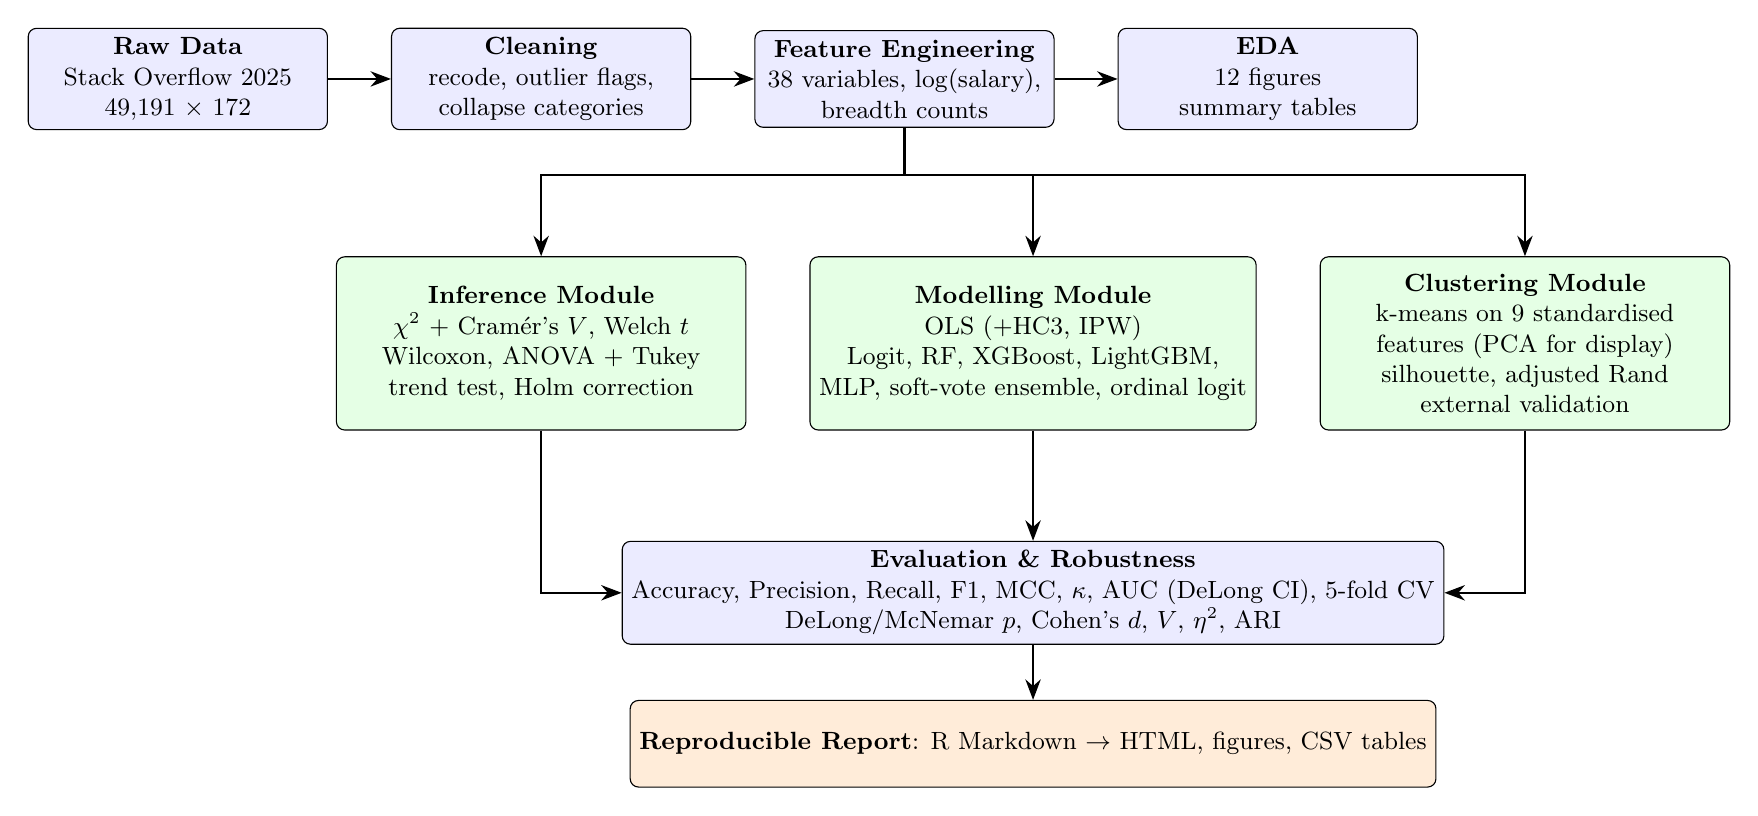
\begin{tikzpicture}[
  node distance=5mm and 8mm,
  blk/.style={draw,rounded corners=3pt,align=center,minimum height=12mm,minimum width=38mm,font=\small,fill=blue!8},
  mod/.style={draw,rounded corners=3pt,align=center,minimum height=22mm,minimum width=52mm,font=\small,fill=green!10},
  outb/.style={draw,rounded corners=3pt,align=center,minimum height=11mm,font=\small,fill=orange!15},
  arr/.style={-{Stealth[length=2.6mm]},thick}]
\node[blk] (raw) {\textbf{Raw Data}\\Stack Overflow 2025\\49{,}191 $\times$ 172};
\node[blk,right=of raw] (clean) {\textbf{Cleaning}\\recode, outlier flags,\\collapse categories};
\node[blk,right=of clean] (fe) {\textbf{Feature Engineering}\\38 variables, $\log$(salary),\\breadth counts};
\node[blk,right=of fe] (eda) {\textbf{EDA}\\12 figures\\summary tables};
\node[mod,below=16mm of clean] (inf) {\textbf{Inference Module}\\$\chi^2$ + Cram\'er's $V$, Welch $t$\\Wilcoxon, ANOVA + Tukey\\trend test, Holm correction};
\node[mod,right=of inf] (mdl) {\textbf{Modelling Module}\\OLS (+HC3, IPW)\\Logit, RF, XGBoost, LightGBM,\\MLP, soft-vote ensemble, ordinal logit};
\node[mod,right=of mdl] (clu) {\textbf{Clustering Module}\\k-means on 9 standardised\\features (PCA for display)\\silhouette, adjusted Rand\\external validation};
\node[blk,below=14mm of mdl,minimum width=96mm] (ev) {\textbf{Evaluation \& Robustness}\\Accuracy, Precision, Recall, F1, MCC, $\kappa$, AUC (DeLong CI), 5-fold CV\\DeLong/McNemar $p$, Cohen's $d$, $V$, $\eta^2$, ARI};
\node[outb,below=7mm of ev,minimum width=96mm] (rep) {\textbf{Reproducible Report}: R Markdown $\to$ HTML, figures, CSV tables};
\draw[arr] (raw)--(clean); \draw[arr] (clean)--(fe); \draw[arr] (fe)--(eda);
\draw[arr] (fe.south) -- ++(0,-6mm) -| (inf.north);
\draw[arr] (fe.south) -- ++(0,-6mm) -| (mdl.north);
\draw[arr] (fe.south) -- ++(0,-6mm) -| (clu.north);
\draw[arr] (inf.south) |- (ev.west);
\draw[arr] (mdl.south) -- (ev.north);
\draw[arr] (clu.south) |- (ev.east);
\draw[arr] (ev)--(rep);
\end{tikzpicture}}
\caption{Architecture of the proposed analysis framework.}
\label{fig:arch}
\end{figure*}

\subsection{Workflow}
Fig.~\ref{fig:flow} shows the end-to-end workflow. Script 01 writes the cleaned dataset, and scripts 02 to 06 each read it directly, so any stage can be re-run on its own. Robust alternatives are computed alongside the standard methods (Wilcoxon rank-sum next to Welch $t$, HC3 errors next to classical OLS errors), and the assumption checks decide which result is relied on. The $p$-values of the hypothesis tests are Holm-adjusted across all eight tests.

\begin{figure}[t]
\centering
\resizebox{0.95\columnwidth}{!}{%
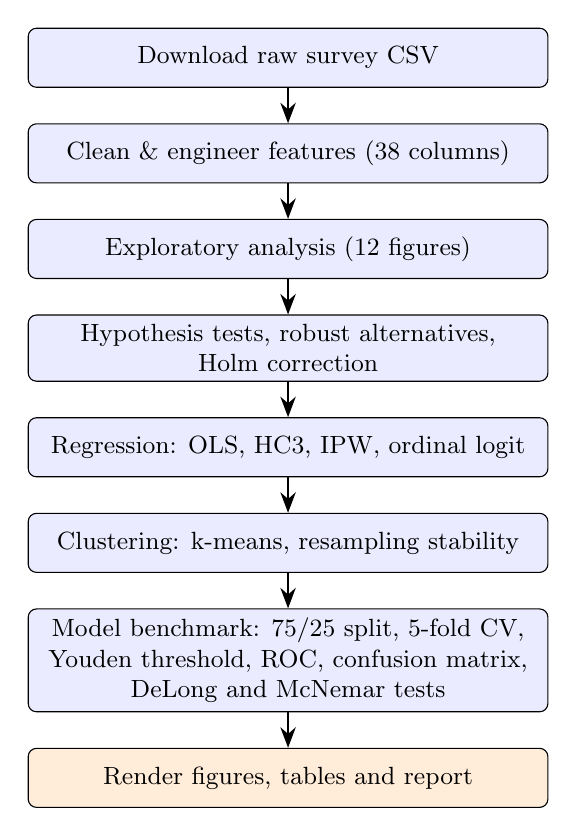
\begin{tikzpicture}[
  node distance=4.5mm,
  st/.style={draw,rounded corners=3pt,align=center,minimum width=66mm,minimum height=7.5mm,font=\small,fill=blue!8},
  arr/.style={-{Stealth[length=2.6mm]},thick}]
\node[st] (a) {Download raw survey CSV};
\node[st,below=of a] (b) {Clean \& engineer features (38 columns)};
\node[st,below=of b] (c) {Exploratory analysis (12 figures)};
\node[st,below=of c] (d) {Hypothesis tests, robust alternatives,\\Holm correction};
\node[st,below=of d] (e) {Regression: OLS, HC3, IPW, ordinal logit};
\node[st,below=of e] (f) {Clustering: k-means, resampling stability};
\node[st,below=of f] (g) {Model benchmark: 75/25 split, 5-fold CV,\\Youden threshold, ROC, confusion matrix,\\DeLong and McNemar tests};
\node[st,below=of g,fill=orange!15] (h) {Render figures, tables and report};
\draw[arr] (a)--(b); \draw[arr] (b)--(c); \draw[arr] (c)--(d); \draw[arr] (d)--(e);
\draw[arr] (e)--(f); \draw[arr] (f)--(g); \draw[arr] (g)--(h);
\end{tikzpicture}}
\caption{Workflow of the project, from raw survey data to the final report.}
\label{fig:flow}
\end{figure}

\subsection{Statistical Inference}
For a two-group comparison, Cohen's $d$ is
\begin{equation}
d=\frac{\bar{x}_1-\bar{x}_2}{s_p},\quad s_p=\sqrt{\frac{(n_1-1)s_1^2+(n_2-1)s_2^2}{n_1+n_2-2}},
\end{equation}
and for an $r\times c$ contingency table Cram\'er's $V$ is
\begin{equation}
V=\sqrt{\frac{\chi^2}{n\,(\min(r,c)-1)}}.
\end{equation}
For a set of $m$ tests, sorted $p$-values $p_{(1)}\le\dots\le p_{(m)}$ are adjusted by Holm's procedure,
\begin{equation}
\tilde p_{(i)}=\max_{j\le i}\min\{1,\,(m-j+1)\,p_{(j)}\}.
\end{equation}
Assumptions are checked where they apply: the minimum expected cell count for the adoption-by-role $\chi^2$ test, and Shapiro--Wilk tests (on random samples of at most 5{,}000 observations per group) together with a variance-ratio $F$ test for the salary comparison. Every Welch $t$ test is accompanied by a Wilcoxon rank-sum test.

\subsection{Regression Models}
Salary is modelled on respondents with complete data as $\log(\text{salary})=\mathbf{x}^\top\boldsymbol\beta+\varepsilon$ with experience, age, education, region, remote work, organisation size, role, AI use and language breadth as predictors. Because the Breusch--Pagan test rejects constant variance, inference uses the HC3 estimator
\begin{equation}
\widehat{V}_{\text{HC3}}=(X^\top X)^{-1}X^\top\,\mathrm{diag}\!\left(\frac{\hat e_i^2}{(1-h_{ii})^2}\right)X\,(X^\top X)^{-1},
\end{equation}
where $h_{ii}$ is the leverage of observation $i$. To check whether missing salaries bias the fit, a response model $\hat\pi_i=P(\text{reports salary}\mid\mathbf{x}_i)$ is estimated and the salary model is refitted with weights $w_i=1/\hat\pi_i$, trimmed at the 99th percentile.

Trust $Y\in\{1,\dots,5\}$ is modelled with the proportional-odds model,
\begin{equation}
\log\frac{P(Y\le j)}{P(Y>j)}=\theta_j-\mathbf{x}^\top\boldsymbol\beta,\quad j=1,\dots,4,
\end{equation}
so that $e^{\beta}$ is the odds ratio for a higher trust rating. The common-slope assumption is checked by fitting a separate binary logit at each cut-point.

\subsection{Predictive Models for AI Adoption (RQ4)}
About \posShare\% of the modelling sample uses AI tools, so a default threshold of 0.5 makes a model predict the majority class almost every time. The decision threshold of each model is therefore chosen with Youden's $J$ \cite{youden1950},
\begin{equation}
J=\max_t\,\bigl[\mathrm{TPR}(t)-\mathrm{FPR}(t)\bigr],
\end{equation}
computed on out-of-fold training predictions and then applied unchanged to the held-out test set. Six models are benchmarked on identical data:
\begin{itemize}
\item \textbf{Logistic regression} (baseline), $P(y{=}1\mid\mathbf{x})=\sigma(\mathbf{x}^\top\boldsymbol\beta)$ \cite{hosmer2013}.
\item \textbf{Random forest}, 500 trees with probability outputs \cite{breiman2001,wright2017}.
\item \textbf{XGBoost}, additive trees minimising the regularised objective \cite{chen2016}
\begin{equation}
\mathcal{L}=\sum_i \ell(y_i,\hat y_i)+\sum_k\bigl[\gamma T_k+\tfrac12\lambda\lVert w_k\rVert^2\bigr],
\end{equation}
with 300 rounds, learning rate 0.05, depth 3, row and column subsampling of 0.8 and minimum child weight 5.
\item \textbf{LightGBM}, histogram-based leaf-wise boosted trees \cite{ke2017} with 300 rounds, learning rate 0.05, 15 leaves, at least 40 observations per leaf, and row and feature subsampling of 0.8.
\item \textbf{MLP}, a single-hidden-layer neural network \cite{venables2002} (8 units, weight decay 0.1, at most 300 iterations) on standardised inputs.
\item \textbf{Soft-voting ensemble}, the mean of the five base models' probabilities,
\begin{equation}
\hat p_{\text{ens}}(\mathbf{x})=\frac1M\sum_{m=1}^{M}\hat p_m(\mathbf{x}).
\end{equation}
\end{itemize}
Only respondents with complete predictor data are modelled, because job satisfaction, language breadth and the AI-threat answer are missing for 40.3\%, 34.3\% and 25.8\% of respondents. The complete cases from the 44{,}682 professionals are divided by one stratified 75/25 split into \nTrain{} training and \nTest{} test respondents. All models use this split, the same predictors (Table~\ref{tab:features}) and fixed hyper-parameters. Algorithm~\ref{alg:bench} summarises the protocol.

\begin{algorithm}[t]
\caption{Model benchmark protocol}
\label{alg:bench}
\begin{algorithmic}[1]
\Require Cleaned survey data $D$, model set $\mathcal{M}$, seed $s$
\Ensure Metrics, ROC curves, confusion matrices, $p$-values
\State Select predictors, drop incomplete rows, set seed $s$
\State Stratified 75/25 split of $D$ on the adoption label
\For{each model $m\in\mathcal{M}$}
  \State Split training set into 5 folds; fit on 4, predict the 5th
  \State Collect out-of-fold probabilities $\hat p^{\text{oof}}_m$
  \State $t_m\gets\arg\max_t J(t)$ on $\hat p^{\text{oof}}_m$ \Comment{Youden}
  \State Fit $m$ on the full training set; predict test set $\hat p_m$
  \State Confusion matrix and metrics at threshold $t_m$
\EndFor
\State Add soft-voting ensemble over all base models $m\in\mathcal{M}$
\State DeLong CI/test and McNemar test of each model vs.\ baseline
\State Holm-adjust the DeLong $p$-values
\State \Return metrics, ROC curves, tables
\end{algorithmic}
\end{algorithm}

\subsection{Clustering (RQ5)}
Nine standardised variables are clustered: years of coding, age, job satisfaction, number of languages, AI sentiment, AI trust, daily AI use, AI-agent use and whether AI handles complex tasks well. The 18{,}638 respondents with complete values on all nine are used. The k-means algorithm \cite{macqueen1967}, which minimises $\sum_{c}\sum_{x\in C_c}\lVert x-\mu_c\rVert^2$, is run for $k=2,\dots,8$ with 25 random starts per $k$, and $k$ is chosen by the average silhouette width \cite{rousseeuw1987},
\begin{equation}
s(i)=\frac{b(i)-a(i)}{\max\{a(i),b(i)\}},
\end{equation}
computed on a random subsample of 2{,}000 respondents because the calculation grows quadratically with sample size. An elbow plot of the within-cluster sum of squares is a cross-check, and the final solution uses 50 random starts. PCA is applied to the same matrix only for a scree plot and a two-dimensional view of the clusters, not as an input to k-means. Reproducibility is measured by the adjusted Rand index (ARI) between the full solution and 25 runs on random 80\% subsamples, each with 25 starts. The clusters are then compared on variables that were left out of the clustering: median salary, remote-work share, large-organisation share and the share answering ``Yes'' to the AI-threat question.

\subsection{Evaluation Metrics}
Classification quality is assessed with
\begin{align}
\text{Accuracy}&=\frac{TP+TN}{TP+TN+FP+FN},\\
\text{Precision}&=\frac{TP}{TP+FP},\\
\text{Recall}&=\frac{TP}{TP+FN},\\
\text{F1}&=\frac{2\cdot\text{Precision}\cdot\text{Recall}}{\text{Precision}+\text{Recall}},
\end{align}
\begin{equation}
\text{MCC}=\frac{TP\,TN-FP\,FN}{\sqrt{(TP{+}FP)(TP{+}FN)(TN{+}FP)(TN{+}FN)}},
\end{equation}
\begin{equation}
\kappa=\frac{p_o-p_e}{1-p_e},
\end{equation}
where $p_o$ is the observed agreement and $p_e$ the agreement expected by chance, together with the area under the ROC curve (AUC). Because the target is imbalanced, accuracy alone is misleading, so MCC, Cohen's $\kappa$ and AUC are reported alongside it.

%==================================================================
\section{Results and Discussion}

\subsection{Descriptive Findings}
Adoption is widespread, but trust is not. Among professional developers who answered each question, 79.4\% use AI tools and 48.1\% use them daily, while only 32.4\% trust the accuracy of the output. Fig.~\ref{fig:eda} shows usage, adoption by experience and trust by experience. Adoption declines from 88.5\% in the 0--2 year group to 72.7\% in the 20+ year group, and over the same range the share who highly or somewhat distrust AI output rises from about 19\% to about 52\%.

\begin{figure*}[t]
\centering
\begin{minipage}{0.32\textwidth}\centering
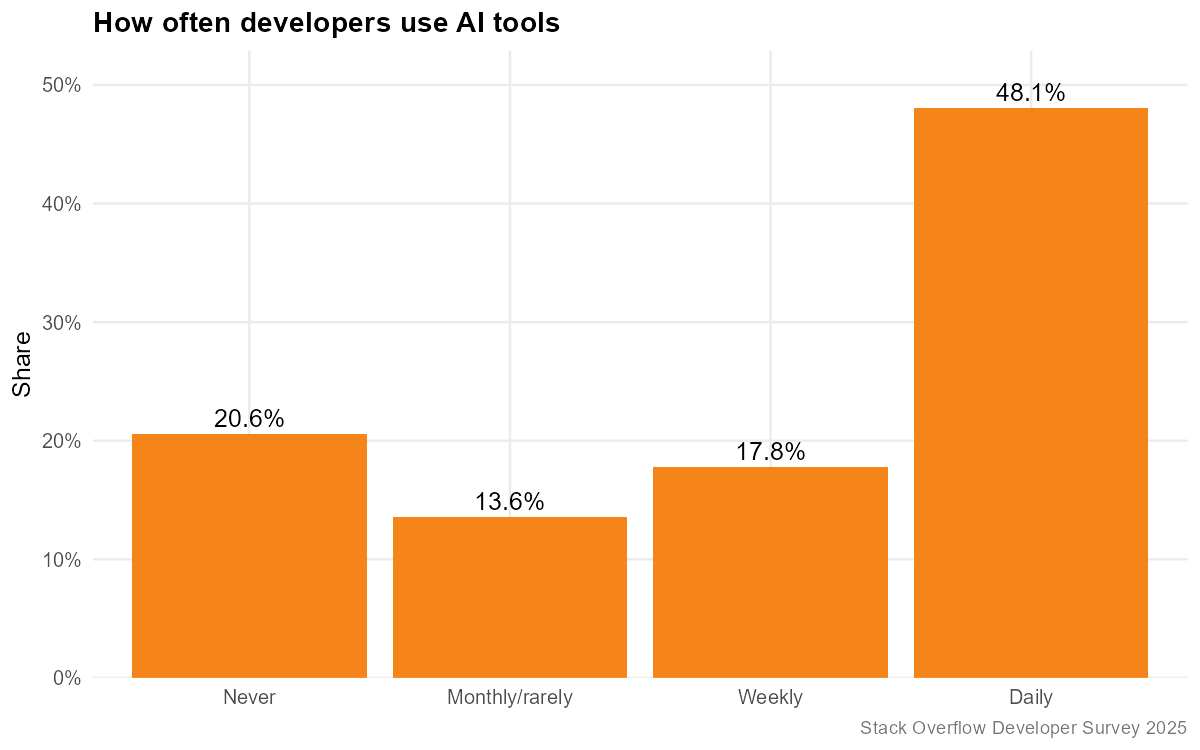
\includegraphics[width=\linewidth]{figures/04_ai_usage.png}\\{\footnotesize (a) AI tool usage}\end{minipage}\hfill
\begin{minipage}{0.32\textwidth}\centering
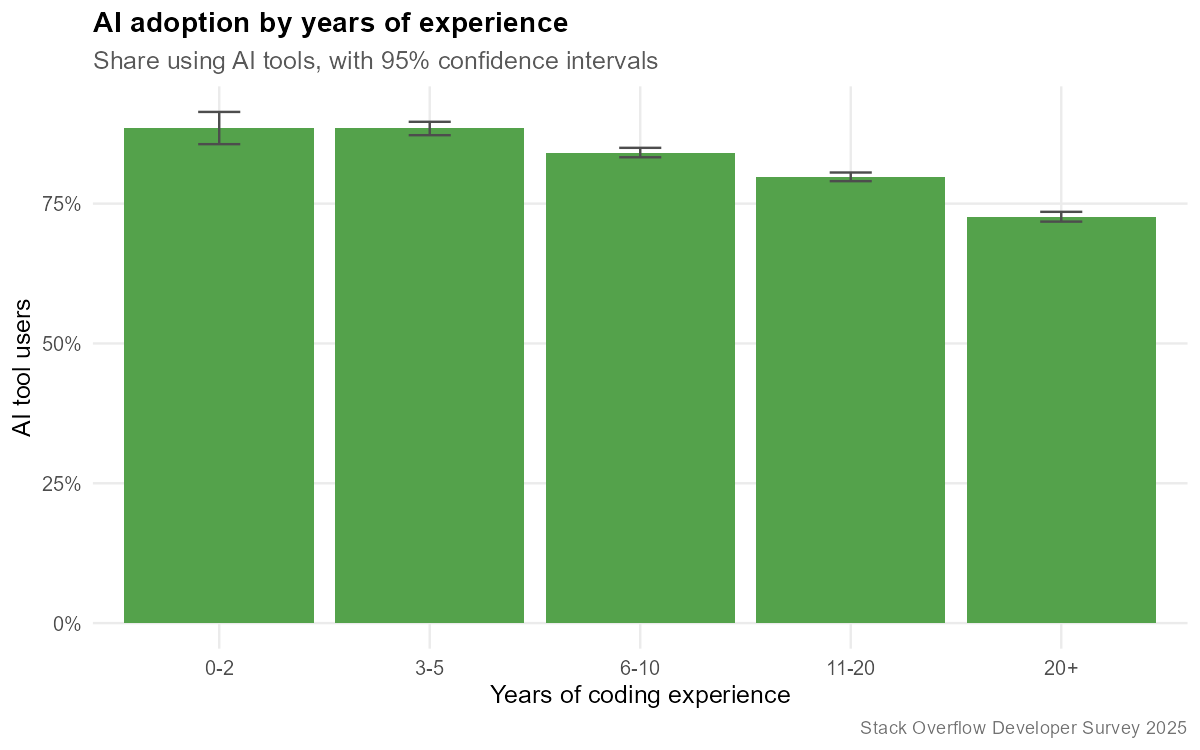
\includegraphics[width=\linewidth]{figures/05_adoption_by_experience.png}\\{\footnotesize (b) Adoption by experience}\end{minipage}\hfill
\begin{minipage}{0.32\textwidth}\centering
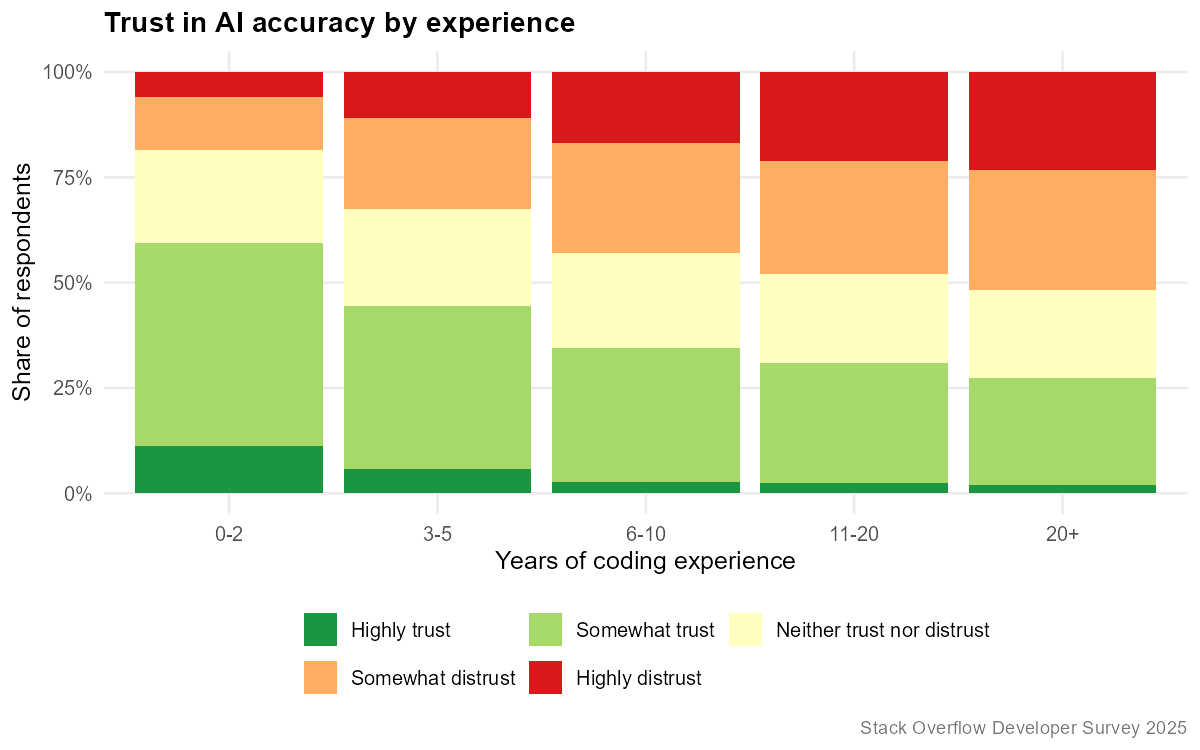
\includegraphics[width=\linewidth]{figures/06_trust_by_experience.png}\\{\footnotesize (c) Trust by experience}\end{minipage}
\caption{Exploratory results: (a) AI usage frequency, (b) adoption by years of experience, (c) trust in AI accuracy by years of experience.}
\label{fig:eda}
\end{figure*}

\subsection{Hypothesis Testing and \texorpdfstring{$p$}{p}-value Analysis}
Table~\ref{tab:pval} reports eight tests addressing six hypotheses, with effect sizes and Holm-adjusted $p$-values. All remain significant after adjustment, which is expected with samples in the tens of thousands, so the effect sizes matter more. Adoption depends on developer role (Cram\'er's $V=0.177$), and trust depends on experience ($V=0.124$, trend statistic 403.7); both are modest effects. AI users earn less than non-users, not more: the median salary is \$76{,}097 for users and \$81{,}685 for non-users (Welch $t$ on log salary, $d=-0.164$, a small effect). The salary reporting rate varies considerably by region ($V=0.168$), so missing salaries cannot be treated as random.

\begin{table*}[t]
\caption{Hypothesis tests: statistics, effect sizes and $p$-values (Holm-adjusted)}
\label{tab:pval}
\centering
\small
\begin{tabular}{p{6.2cm}rrp{3.6cm}cc}
\toprule
\textbf{Hypothesis} & \textbf{Stat.} & \textbf{df} & \textbf{Effect size} & \textbf{$p$} & \textbf{Holm $p$} \\
\midrule
H1: Adoption vs.\ developer role ($\chi^2$) & 972.2 & 25 & Cram\'er's $V=0.177$ & $<0.001$ & $<0.001$ \\
H2: Salary, AI users vs.\ non-users (Welch $t$) & $-10.8$ & 7{,}488 & Cohen's $d=-0.164$ & $<0.001$ & $<0.001$ \\
H2b: Salary, same (Wilcoxon rank-sum) & 34{,}442{,}132 & -- & rank-biserial $r=-0.068$ & $<0.001$ & $<0.001$ \\
H3: Salary across education (ANOVA) & 82.6 & 3 & $\eta^2=0.011$ & $<0.001$ & $<0.001$ \\
H4: Trust vs.\ experience ($\chi^2$) & 465.8 & 4 & Cram\'er's $V=0.124$ & $<0.001$ & $<0.001$ \\
H4b: Trust vs.\ experience (trend test) & 403.7 & 1 & -- & $<0.001$ & $<0.001$ \\
H5: Job satisfaction, daily AI users vs.\ others (Wilcoxon) & 80{,}974{,}594 & -- & rank-biserial $r=0.043$ & $<0.001$ & $<0.001$ \\
H6: Salary response vs.\ region ($\chi^2$) & 920.0 & 6 & Cram\'er's $V=0.168$ & $<0.001$ & $<0.001$ \\
\bottomrule
\end{tabular}
\end{table*}

\subsection{Regression Analysis}
The linear model for $\log$(salary) is fitted on 17{,}940 respondents with complete data and reaches $R^2=0.443$. Region has the largest coefficients: relative to Africa, North America, Oceania and Europe are higher by 1.71, 1.33 and 1.04 log points. Developer role follows, with coefficients up to 0.88 for senior executives and 0.80 for engineering managers relative to academic researchers, then organisation size and education. Relative to respondents with no degree, a doctorate or professional degree is associated with about 31\% higher salary after adjustment (coefficient 0.267) and about 49\% higher salary in the unadjusted pairwise Tukey comparison ($p<0.001$). The AI-use coefficient is 0.018 log points (95\% CI $-0.011$ to $0.047$, $p=0.23$; $p=0.17$ with HC3 errors), which cannot be distinguished from zero. The raw salary gap between AI users and non-users therefore does not remain once experience, region and the other covariates are controlled.

The Breusch--Pagan test rejects constant variance (BP $=1043.6$, $p<0.001$), so conclusions use HC3 standard errors, which are on average $1.13\times$ the classical ones (region coefficients rise by 1.3 to 1.5 times). Two coefficients lose significance at the 5\% level under the robust errors: the QA or test role and the retired category. Only 52.1\% of respondents report salary. Refitting with inverse-probability weights changes the coefficients by a median of 0.0036 log points (largest change about 0.02, for the data or business analyst role), and the AI-use coefficient moves from 0.0176 to 0.0205, so the complete-case results are stable.

\subsection{Ordinal Model of Trust (RQ6)}
The proportional-odds model for the full five-point trust scale ($n=19{,}112$) shows that usage frequency is the strongest predictor. Compared with respondents who do not currently use AI tools (including those who plan to), daily users have 11.2 times the odds of a higher trust rating (95\% CI 10.3--12.1), weekly users 5.3 times and monthly or rare users 2.4 times. Each additional year of coding multiplies the odds by 0.969, which is about 27\% lower over a decade, while age has a small positive association once experience is held constant. Region is also strongly associated with trust: relative to Africa, respondents in Europe, North America and Oceania have odds of a higher rating of 0.40, 0.35 and 0.33 times. The association with usage may run in both directions, and the model cannot separate them. In the proportional-odds check, 10 of the 46 coefficients vary more across cut-points than their own size. Four are role categories (retired, senior executives, ``other'' and cloud infrastructure engineers) and six are terms whose average effect is close to zero (Asia and Middle East, bachelor's degree, doctorate, medium and large organisations, and language count). The terms on which the conclusions rest (usage frequency, years of coding, age, and the North America, Europe and Oceania contrasts) are all stable across cut-points.

\subsection{Confusion-Matrix Analysis of Adoption Prediction (RQ4)}
Table~\ref{tab:cm} gives the confusion-matrix counts on the \nTest{} held-out respondents, Table~\ref{tab:metrics} the derived metrics, and Fig.~\ref{fig:cm} the row-normalised matrices. Because \posShare\% of respondents use AI tools, a classifier that always predicts ``adopter'' already reaches an accuracy of \baselineAcc. Every model falls below this accuracy (Table~\ref{tab:metrics}). This is by design: the Youden threshold gives up accuracy to identify non-users, so accuracy cannot be used to rank the models, and the comparison rests on AUC, MCC and $\kappa$.

On those measures the best model is \bestModel{} (AUC \bestAUC, 95\% CI \bestAUCci; recall \bestRecall, specificity \bestSpec, MCC \bestMCC), but the performance is weak in absolute terms. MCC and $\kappa$ are both low for all six models (Table~\ref{tab:metrics}), which indicates only slight agreement beyond chance. Precision lies between 0.855 and 0.884, only 4 to 7 points above the \posShare\% base rate, so a predicted adopter is only marginally more likely to be a true adopter than a random respondent. The MLP has the highest accuracy, recall and F1, yet has one of the two lowest AUCs. It reaches those values by labelling more respondents as adopters than any other model does (Table~\ref{tab:cm}), which is a threshold effect and not better ranking. Cross-validated AUCs on the training folds are within 0.01 of the test AUCs for every model (Table~\ref{tab:metrics}), so the weak result is not an artefact of a single split. For reference, logistic regression reaches an AUC of \lrAUC{} and the random forest \rfAUC.

\begin{table}[t]
\caption{Confusion-matrix counts on the held-out test set (Youden threshold from training predictions)}
\label{tab:cm}
\centering
\small
\begin{tabular}{lccccc}
\toprule
\textbf{Model} & \textbf{Thr.} & \textbf{TN} & \textbf{FP} & \textbf{FN} & \textbf{TP} \\
\midrule
Logistic regression & 0.82 & 594 & 311 & 1683 & 2215 \\
Random forest & 0.79 & 494 & 411 & 1474 & 2424 \\
XGBoost & 0.82 & 625 & 280 & 1763 & 2135 \\
LightGBM & 0.82 & 594 & 311 & 1661 & 2237 \\
MLP (nnet) & 0.80 & 480 & 425 & 1290 & 2608 \\
Ensemble (soft vote) & 0.81 & 574 & 331 & 1538 & 2360 \\
\bottomrule
\end{tabular}

\end{table}

\begin{table*}[t]
\caption{Classification performance on the held-out test set (best value per column in bold; CV-AUC is the mean AUC over the five training folds)}
\label{tab:metrics}
\centering
\small
\begin{tabular}{lccccccccc}
\toprule
\textbf{Model} & \textbf{Acc.} & \textbf{Prec.} & \textbf{Rec.} & \textbf{Spec.} & \textbf{F1} & \textbf{MCC} & $\boldsymbol{\kappa}$ & \textbf{AUC} & \textbf{CV-AUC} \\
\midrule
Logistic regression & 0.585 & 0.877 & 0.568 & 0.656 & 0.690 & 0.176 & 0.142 & 0.656 & 0.665 \\
Random forest & 0.608 & 0.855 & 0.622 & 0.546 & 0.720 & 0.133 & 0.116 & 0.634 & 0.632 \\
XGBoost & 0.575 & \textbf{0.884} & 0.548 & \textbf{0.691} & 0.676 & 0.186 & 0.146 & \textbf{0.666} & \textbf{0.669} \\
LightGBM & 0.589 & 0.878 & 0.574 & 0.656 & 0.694 & 0.180 & 0.146 & 0.657 & 0.660 \\
MLP (nnet) & \textbf{0.643} & 0.860 & \textbf{0.669} & 0.530 & \textbf{0.753} & 0.162 & 0.146 & 0.634 & 0.627 \\
Ensemble (soft vote) & 0.611 & 0.877 & 0.605 & 0.634 & 0.716 & \textbf{0.189} & \textbf{0.159} & 0.665 & 0.667 \\
\midrule
Majority-class baseline & 0.812 & -- & -- & -- & -- & 0.000 & 0.000 & 0.500 & -- \\
\bottomrule
\end{tabular}

\end{table*}

\begin{figure*}[t]
\centering
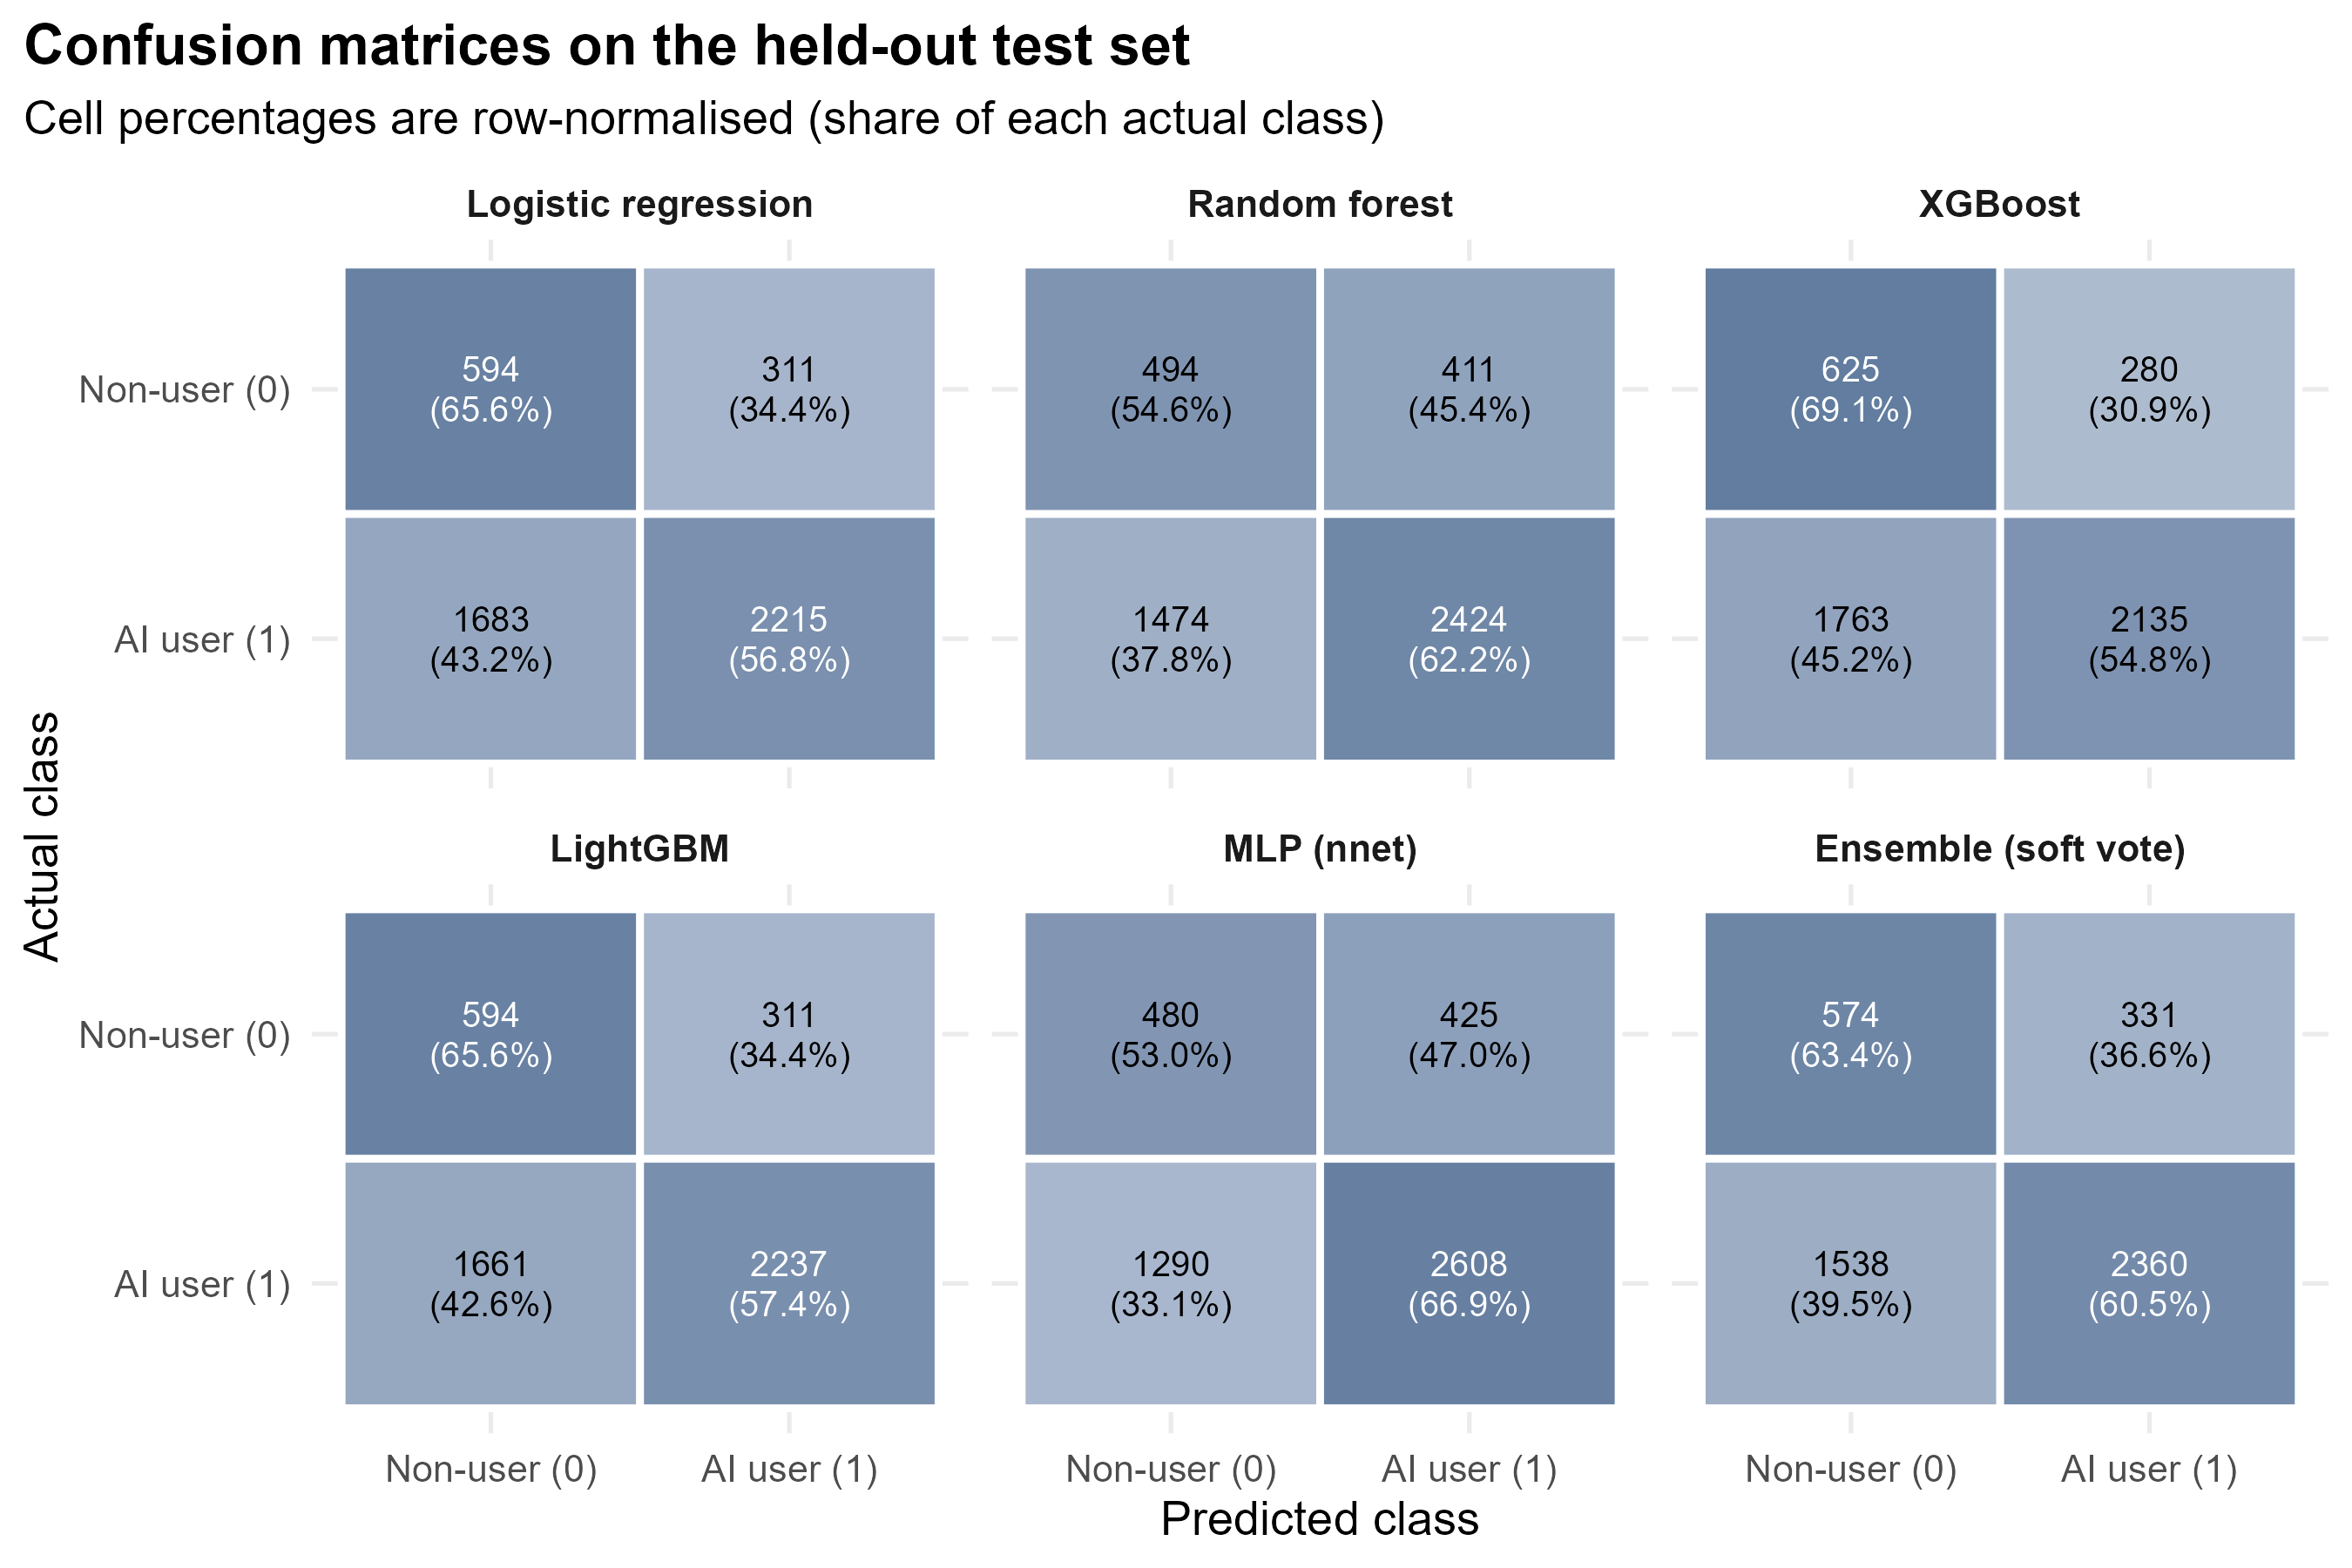
\includegraphics[width=0.62\textwidth]{figures/confusion_matrices.png}
\caption{Row-normalised confusion matrices of the benchmarked models on the held-out test set.}
\label{fig:cm}
\end{figure*}

\subsection{ROC/AUC Analysis}
Fig.~\ref{fig:roc} plots the ROC curves. AUC measures ranking quality independently of the threshold, and the dashed diagonal marks chance level. All curves lie above the diagonal but within a narrow band. With the best AUC at \bestAUC, a randomly chosen adopter is ranked above a randomly chosen non-adopter only about two times in three. Adoption is therefore only weakly separable from the ten professional attributes used as predictors.

\begin{figure}[t]
\centering
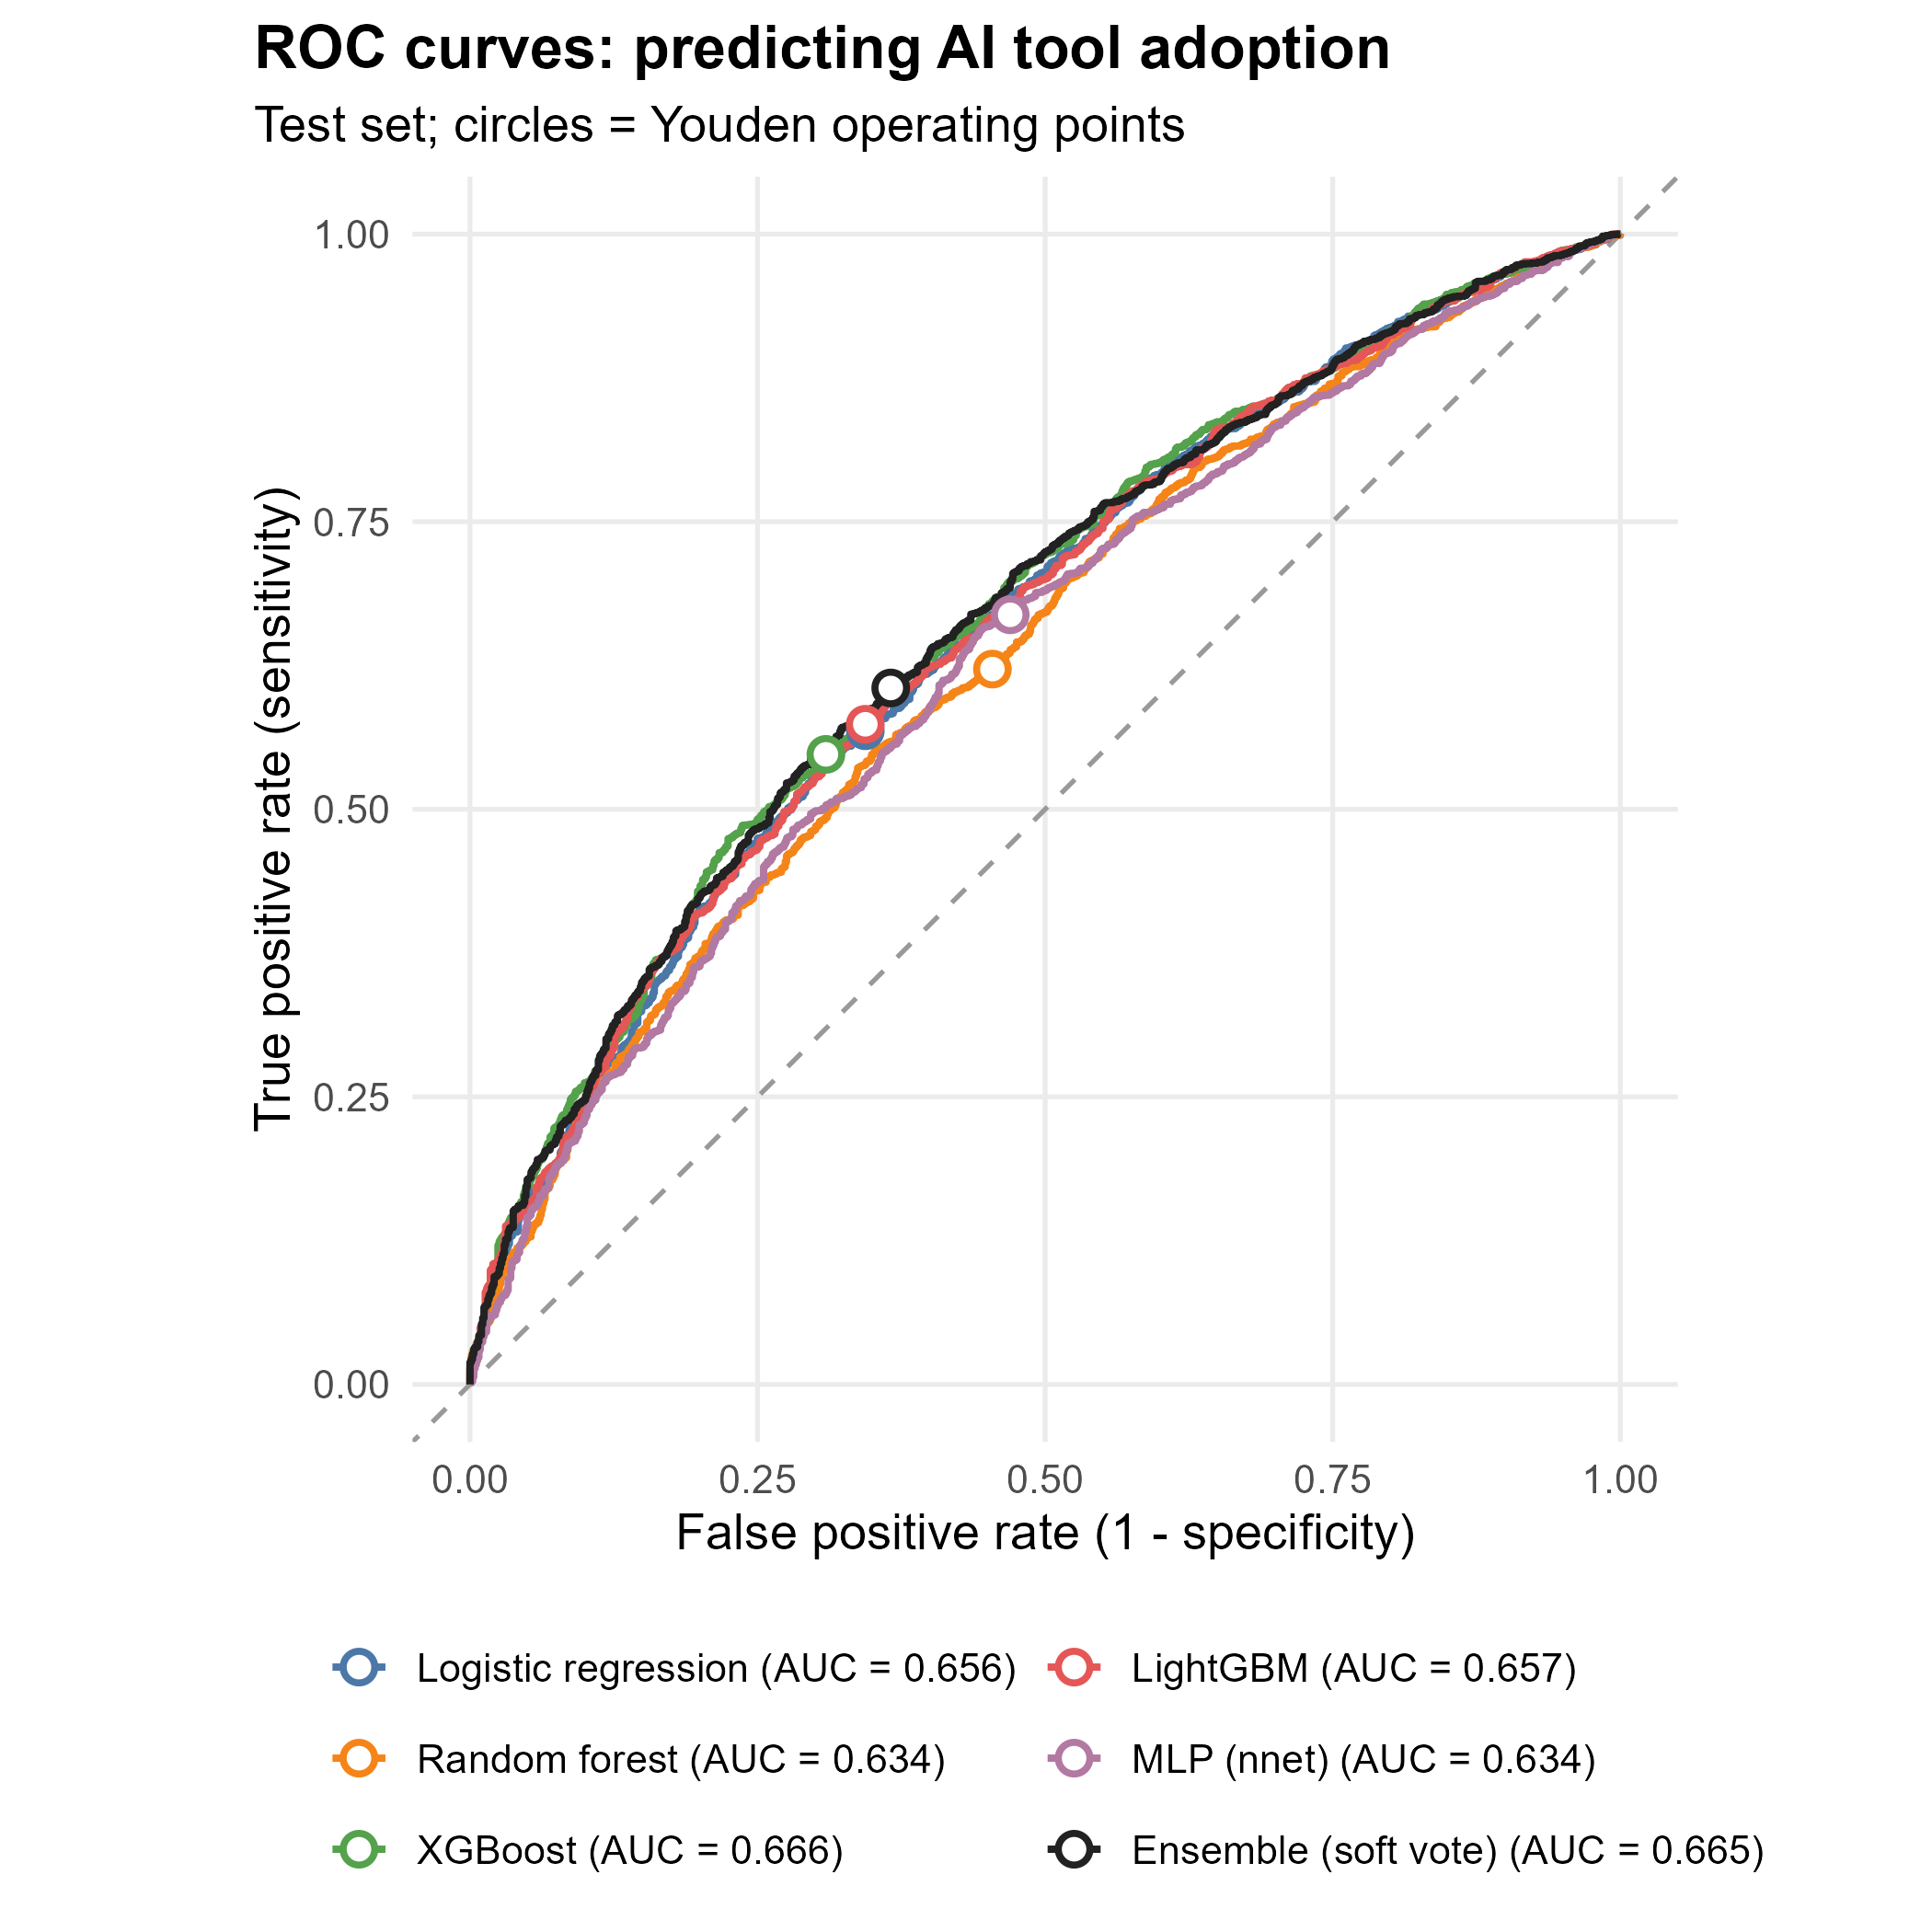
\includegraphics[width=0.78\columnwidth]{figures/roc_comparison.png}
\caption{ROC curves of the benchmarked models for AI-adoption prediction.}
\label{fig:roc}
\end{figure}

\subsection{Significance of Model Differences}
Table~\ref{tab:modelp} tests every model against the logistic-regression baseline on the same test set, using DeLong's test for the difference in AUC and McNemar's test for the paired difference in errors. The random forest and the MLP are reliably \emph{worse} than logistic regression, with Holm-adjusted $p$-values below 0.05. The best model, \bestModel, is nominally better (\bestDeltaAUC, DeLong $p=\bestDeltaP$), but its Holm-adjusted $p$-value in Table~\ref{tab:modelp} is above 0.05, so the advantage is not reliable once the five comparisons are corrected for. LightGBM and the ensemble are likewise statistically indistinguishable from the baseline after correction. In practice, a plain logistic regression does as well as any model tested, and the extra complexity of boosting, neural networks and ensembling brings no reliable improvement here.

The McNemar column must be read separately. It compares errors at each model's own threshold, so it is sensitive to the number of respondents each model labels as adopters (Table~\ref{tab:cm}) as well as to ranking quality. DeLong's test compares discrimination directly and is the comparison on which the conclusions rest.

\begin{table*}[t]
\caption{Pairwise comparison of each model against the logistic-regression baseline: AUC with DeLong 95\% CI, DeLong, Holm-adjusted and McNemar $p$-values}
\label{tab:modelp}
\centering
\small
\begin{tabular}{lccccc}
\toprule
\textbf{Model} & \textbf{AUC [95\% CI]} & $\boldsymbol{\Delta}$\textbf{AUC} & \textbf{DeLong $p$} & \textbf{Holm $p$} & \textbf{McNemar $p$} \\
\midrule
Logistic regression & 0.656 [0.637, 0.676] & ref. & -- & -- & -- \\
Random forest & 0.634 [0.614, 0.654] & -0.022 & 0.010 & 0.041 & 0.003 \\
XGBoost & 0.666 [0.647, 0.685] & +0.010 & 0.042 & 0.127 & 0.042 \\
LightGBM & 0.657 [0.638, 0.676] & +0.001 & 0.870 & 0.870 & 0.427 \\
MLP (nnet) & 0.634 [0.615, 0.654] & -0.022 & 0.002 & 0.010 & $<0.001$ \\
Ensemble (soft vote) & 0.665 [0.646, 0.684] & +0.008 & 0.057 & 0.127 & $<0.001$ \\
\bottomrule
\end{tabular}

\end{table*}

\subsection{Predictors of Trust and Adoption}
Fig.~\ref{fig:drivers} shows the ordinal-model effects for trust (left) and random-forest variable importance for adoption (right). For trust, usage frequency has the largest positive effect, while respondents in Europe, North America and Oceania have markedly lower odds of a higher rating than those in the reference region (Africa); years of coding has a small negative effect per year. For adoption, years of coding and age have by far the highest permutation importance, followed by region and developer role.

\begin{figure}[t]
\centering
\begin{minipage}{0.49\columnwidth}\centering
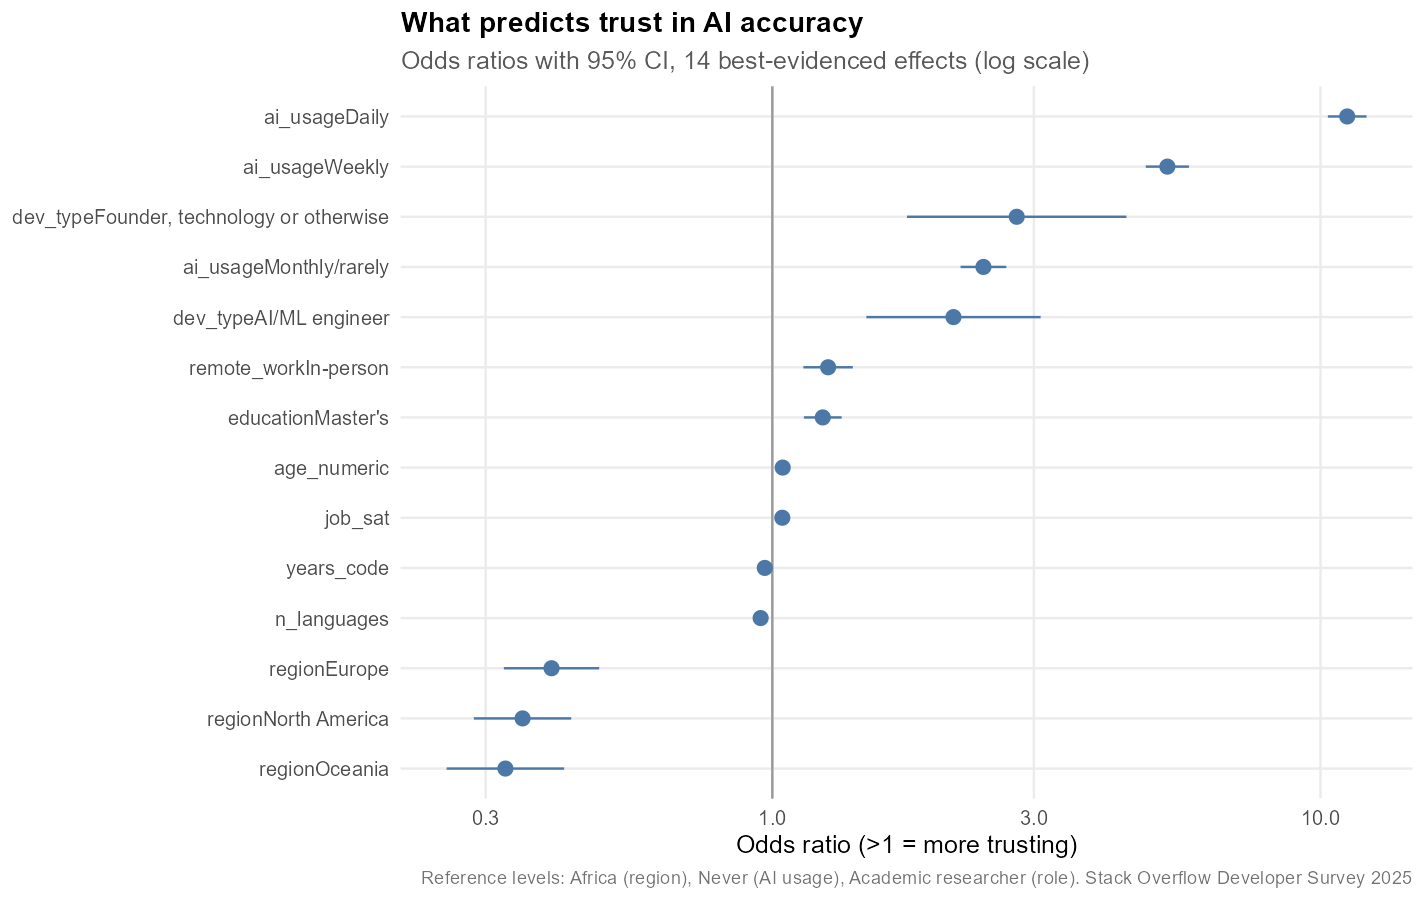
\includegraphics[width=\linewidth]{figures/22_ordinal_trust_effects.png}\\{\footnotesize (a) Ordinal trust effects}\end{minipage}\hfill
\begin{minipage}{0.49\columnwidth}\centering
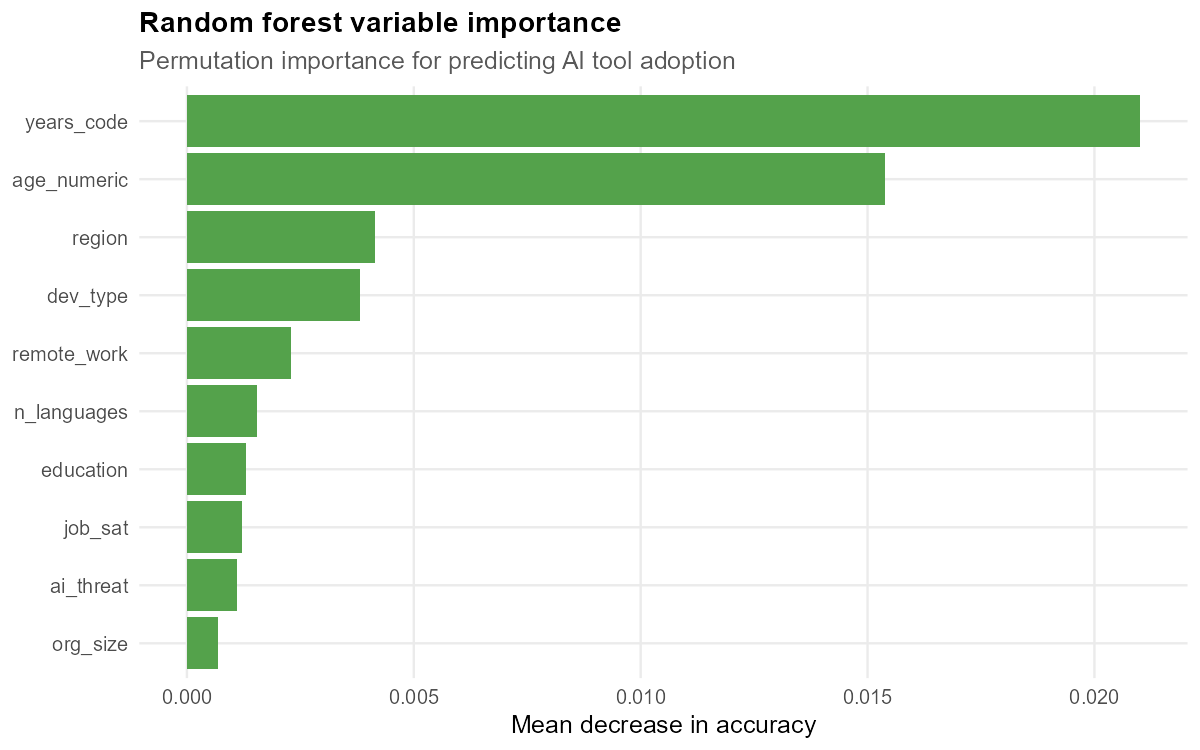
\includegraphics[width=\linewidth]{figures/16_rf_importance.png}\\{\footnotesize (b) RF importance}\end{minipage}
\caption{Drivers of (a) trust in AI accuracy and (b) AI adoption.}
\label{fig:drivers}
\end{figure}

\subsection{Clustering of AI Attitudes (RQ5)}
The average silhouette width is highest at $k=2$ (0.184); for $k=3$ to 8 it lies between 0.151 and 0.177. K-means gives the two groups described in Table~\ref{tab:clusters} and Fig.~\ref{fig:clusters}. The \emph{AI-embracing} cluster (54.5\%) has 87\% daily users and a mean trust score of 3.51 out of 5, whereas the \emph{sceptical} cluster (45.5\%) has 24\% daily users and a mean trust score of 1.95. A silhouette width at or below 0.25 is read as ``no substantial structure'' under the rule of thumb of Kaufman and Rousseeuw \cite{kaufman1990}, so the two groups describe a continuum rather than two clearly separated clusters. The partition is nevertheless highly reproducible: the mean adjusted Rand index is 0.998 (minimum 0.993) over 25 subsample runs. On variables that were not used in the clustering, the sceptical group has the higher median salary (\$83{,}668 against \$73{,}686) and large-organisation share, and the AI-embracing group is more likely to answer ``Yes'' to the AI-threat question (17.3\% against 10.7\%).

\begin{table}[t]
\caption{Cluster profiles (k-means, $k=2$, $n=18{,}638$)}
\label{tab:clusters}
\centering
\small
\begin{tabular}{@{}lcc@{}}
\toprule
\textbf{Property} & \textbf{AI-embracing} & \textbf{Sceptical} \\
\midrule
Share of respondents & 54.5\% & 45.5\% \\
Daily AI users & 87\% & 24\% \\
Mean trust score (1--5) & 3.51 & 1.95 \\
Mean sentiment score (1--5) & 4.42 & 2.98 \\
Uses AI agents & 51\% & 17\% \\
Mean years coding & 16.9 & 18.5 \\
\midrule
\multicolumn{3}{@{}l}{\emph{Not used in the clustering}} \\
Median salary (USD) & 73{,}686 & 83{,}668 \\
Remote work & 36.7\% & 33.9\% \\
Large organisation (1000+) & 29.7\% & 33.7\% \\
AI-threat answer ``Yes'' & 17.3\% & 10.7\% \\
\bottomrule
\end{tabular}
\end{table}

\begin{figure}[t]
\centering
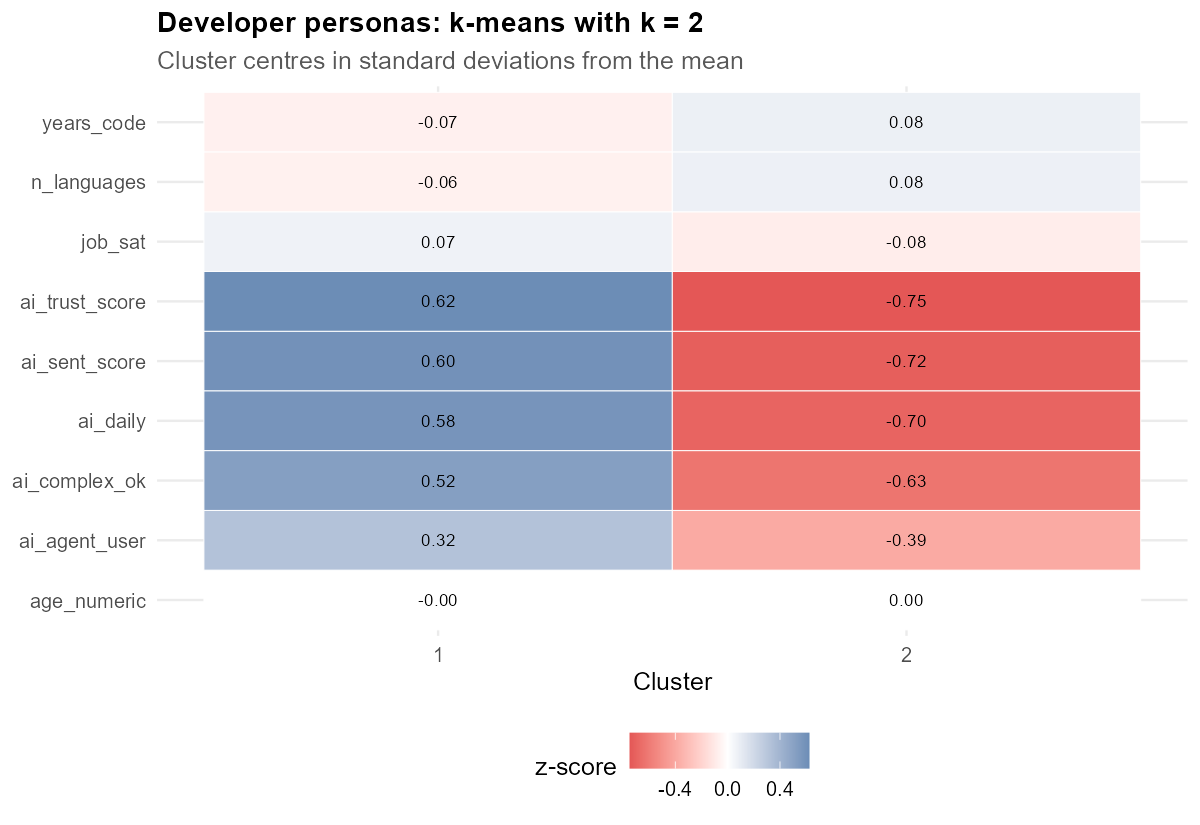
\includegraphics[width=0.8\columnwidth]{figures/20_cluster_centres.png}
\caption{Standardised cluster centres for the two attitude personas.}
\label{fig:clusters}
\end{figure}

\subsection{What Developers Complain About}
The main complaint concerns reliability rather than capability. Among respondents who answered the question, about 67\% name ``AI solutions that are almost right, but not quite'' as a frustration, about 46\% say that debugging AI-generated code takes more time, and about 19\% report becoming less confident in their own problem solving. These complaints concern reliability, which is consistent with the low share of respondents who trust AI accuracy; the survey data cannot show why trust is lowest among the most experienced developers.

\subsection{Robustness Summary}
Table~\ref{tab:robust} lists the checks applied to the headline results.

\begin{table}[t]
\caption{Robustness checks and outcomes}
\label{tab:robust}
\centering
\small
\begin{tabular}{@{}p{2.3cm}p{2.7cm}p{2.5cm}@{}}
\toprule
\textbf{Threat} & \textbf{Check} & \textbf{Outcome} \\
\midrule
Non-constant variance & Breusch--Pagan, HC3 SEs & BP $=1043.6$; SEs $1.13\times$ \\
Missing salaries & IPW refit & median shift 0.0036 \\
Non-normal salary & Wilcoxon, $\log$ model & same direction, $p<0.001$ \\
Proportional odds & per-cut-point logits & key terms stable; 10 of 46 not \\
Weak clusters & silhouette + ARI & 0.184 vs.\ 0.998 \\
Imbalanced target & Youden, MCC, $\kappa$, AUC & accuracy not used alone \\
\bottomrule
\end{tabular}
\end{table}

\subsection{Discussion}
The results point to three main conclusions. First, adoption, trust and pay are separate matters. Almost nine in ten of the least experienced developers use AI tools, yet trust declines with experience, and AI use is not significantly associated with salary once geography, experience, role and education are controlled. Second, statistical significance says little here, because every test is significant. The effect sizes ($d=-0.16$, $V$ between 0.12 and 0.18) show that most differences are modest, and the large associations are those of usage frequency and region with trust. Third, adoption is only weakly predictable: the best AUC is \bestAUC{} against \lrAUC{} for logistic regression, MCC is low for every model (Table~\ref{tab:metrics}), and after Holm correction no model is reliably better than the baseline (Table~\ref{tab:modelp}). Role (Table~\ref{tab:pval}) and experience (Fig.~\ref{fig:eda}b) are associated with adoption, but the recorded attributes do not identify \emph{which individual} adopts.

%==================================================================
\section{Limitations}
The sample consists of self-selected survey respondents, and about 73\% of those with a known region are in Europe or North America, so the results should not be generalised to all developers. The data are cross-sectional, so every result is an association; in particular, the lower raw salary of AI users says nothing about the effect of AI itself. Respondents who plan to adopt AI are counted as non-users. Salary is self-reported and depends on exchange rates, and collapsing 175 countries into seven regions loses variation. The adoption benchmark uses only complete cases (\nTrain{} training and \nTest{} test respondents, from 44{,}682 professionals), which may not represent respondents who skipped the satisfaction or language questions. It also uses fixed hyper-parameters on a single stratified split, and its decision thresholds are tuned for balanced sensitivity and specificity, which lowers accuracy below the majority-class baseline. CatBoost and deep tabular models (FT-Transformer, TabPFN) are discussed but not benchmarked here.

\section{Conclusion and Future Work}
This paper analysed the Stack Overflow Developer Survey 2025 with a reproducible statistical and machine-learning pipeline. AI adoption among professional developers is very high, but trust is much lower and declines with experience, and AI use is not significantly associated with pay once experience, region and the other covariates are controlled. Adoption is only weakly predictable (best AUC \bestAUC, low MCC for every model), and no benchmarked model is reliably better than logistic regression after multiple-comparison correction. Two reproducible attitude groups separate developers who embrace AI from those who doubt it. Future work will benchmark tuned gradient boosting, CatBoost and tabular transformers (FT-Transformer, TabPFN), add SHAP-based explanations, repeat the analysis on earlier survey years, and test causal designs such as matching or instrumental variables.

%==================================================================
\begin{thebibliography}{99}
\bibitem{peng2023} S. Peng, E. Kalliamvakou, P. Cihon, and M. Demirer, ``The impact of AI on developer productivity: Evidence from GitHub Copilot,'' arXiv:2302.06590, 2023.
\bibitem{so2025} Stack Overflow, ``Annual Developer Survey 2025,'' 2025. [Online]. Available: https://survey.stackoverflow.co/
\bibitem{cohen1988} J. Cohen, \emph{Statistical Power Analysis for the Behavioral Sciences}, 2nd ed. Hillsdale, NJ, USA: Lawrence Erlbaum, 1988.
\bibitem{holm1979} S. Holm, ``A simple sequentially rejective multiple test procedure,'' \emph{Scand. J. Statist.}, vol. 6, no. 2, pp. 65--70, 1979.
\bibitem{breusch1979} T. S. Breusch and A. R. Pagan, ``A simple test for heteroscedasticity and random coefficient variation,'' \emph{Econometrica}, vol. 47, no. 5, pp. 1287--1294, 1979.
\bibitem{white1980} H. White, ``A heteroskedasticity-consistent covariance matrix estimator and a direct test for heteroskedasticity,'' \emph{Econometrica}, vol. 48, no. 4, pp. 817--838, 1980.
\bibitem{mackinnon1985} J. G. MacKinnon and H. White, ``Some heteroskedasticity-consistent covariance matrix estimators with improved finite sample properties,'' \emph{J. Econometrics}, vol. 29, no. 3, pp. 305--325, 1985.
\bibitem{mccullagh1980} P. McCullagh, ``Regression models for ordinal data,'' \emph{J. Roy. Statist. Soc. B}, vol. 42, no. 2, pp. 109--142, 1980.
\bibitem{agresti2010} A. Agresti, \emph{Analysis of Ordinal Categorical Data}, 2nd ed. Hoboken, NJ, USA: Wiley, 2010.
\bibitem{seaman2013} S. R. Seaman and I. R. White, ``Review of inverse probability weighting for dealing with missing data,'' \emph{Statist. Methods Med. Res.}, vol. 22, no. 3, pp. 278--295, 2013.
\bibitem{breiman2001} L. Breiman, ``Random forests,'' \emph{Mach. Learn.}, vol. 45, no. 1, pp. 5--32, 2001.
\bibitem{chen2016} T. Chen and C. Guestrin, ``XGBoost: A scalable tree boosting system,'' in \emph{Proc. ACM SIGKDD}, 2016, pp. 785--794.
\bibitem{ke2017} G. Ke \emph{et al.}, ``LightGBM: A highly efficient gradient boosting decision tree,'' in \emph{Proc. NeurIPS}, 2017, pp. 3146--3154.
\bibitem{prokhorenkova2018} L. Prokhorenkova, G. Gusev, A. Vorobev, A. V. Dorogush, and A. Gulin, ``CatBoost: Unbiased boosting with categorical features,'' in \emph{Proc. NeurIPS}, 2018, pp. 6638--6648.
\bibitem{grinsztajn2022} L. Grinsztajn, E. Oyallon, and G. Varoquaux, ``Why do tree-based models still outperform deep learning on typical tabular data?'' in \emph{Proc. NeurIPS Datasets and Benchmarks}, 2022.
\bibitem{shwartz2022} R. Shwartz-Ziv and A. Armon, ``Tabular data: Deep learning is not all you need,'' \emph{Inf. Fusion}, vol. 81, pp. 84--90, 2022.
\bibitem{gorishniy2021} Y. Gorishniy, I. Rubachev, V. Khrulkov, and A. Babenko, ``Revisiting deep learning models for tabular data,'' in \emph{Proc. NeurIPS}, 2021, pp. 18932--18943.
\bibitem{huang2020} X. Huang, A. Khetan, M. Cvitkovic, and Z. Karnin, ``TabTransformer: Tabular data modeling using contextual embeddings,'' arXiv:2012.06678, 2020.
\bibitem{hollmann2025} N. Hollmann \emph{et al.}, ``Accurate predictions on small data with a tabular foundation model,'' \emph{Nature}, vol. 637, pp. 319--326, 2025.
\bibitem{fawcett2006} T. Fawcett, ``An introduction to ROC analysis,'' \emph{Pattern Recognit. Lett.}, vol. 27, no. 8, pp. 861--874, 2006.
\bibitem{delong1988} E. R. DeLong, D. M. DeLong, and D. L. Clarke-Pearson, ``Comparing the areas under two or more correlated receiver operating characteristic curves: A nonparametric approach,'' \emph{Biometrics}, vol. 44, no. 3, pp. 837--845, 1988.
\bibitem{mcnemar1947} Q. McNemar, ``Note on the sampling error of the difference between correlated proportions or percentages,'' \emph{Psychometrika}, vol. 12, no. 2, pp. 153--157, 1947.
\bibitem{macqueen1967} J. MacQueen, ``Some methods for classification and analysis of multivariate observations,'' in \emph{Proc. 5th Berkeley Symp. Math. Statist. Probab.}, vol. 1, 1967, pp. 281--297.
\bibitem{rousseeuw1987} P. J. Rousseeuw, ``Silhouettes: A graphical aid to the interpretation and validation of cluster analysis,'' \emph{J. Comput. Appl. Math.}, vol. 20, pp. 53--65, 1987.
\bibitem{hubert1985} L. Hubert and P. Arabie, ``Comparing partitions,'' \emph{J. Classification}, vol. 2, no. 1, pp. 193--218, 1985.
\bibitem{youden1950} W. J. Youden, ``Index for rating diagnostic tests,'' \emph{Cancer}, vol. 3, no. 1, pp. 32--35, 1950.
\bibitem{hosmer2013} D. W. Hosmer, S. Lemeshow, and R. X. Sturdivant, \emph{Applied Logistic Regression}, 3rd ed. Hoboken, NJ, USA: Wiley, 2013.
\bibitem{wright2017} M. N. Wright and A. Ziegler, ``ranger: A fast implementation of random forests for high dimensional data in C++ and R,'' \emph{J. Statist. Softw.}, vol. 77, no. 1, pp. 1--17, 2017.
\bibitem{venables2002} W. N. Venables and B. D. Ripley, \emph{Modern Applied Statistics with S}, 4th ed. New York, NY, USA: Springer, 2002.
\bibitem{kaufman1990} L. Kaufman and P. J. Rousseeuw, \emph{Finding Groups in Data: An Introduction to Cluster Analysis}. Hoboken, NJ, USA: Wiley, 1990.
\end{thebibliography}

\end{document}
